\chapter {Controlling Single Board Heater System by PID controller}
The aim of this experiment is to apply a PID controller to the single board heater system. The target group is anyone who has basic knowledge of Control Engineering.
\begin{figure}
\centering
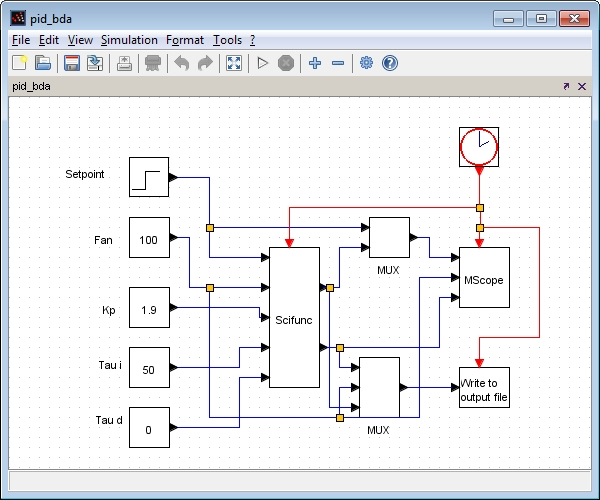
\includegraphics[width=0.7\linewidth]{pid_manual/pid_xcos.jpg}
\caption{Xcos interface for this experiment}
\label{Xcos_pid}
\end{figure}
We have used Scilab with Xcos as an interface for sending and receiving data. This interface is shown in Fig.\ref{Xcos_pid}. Heater current and fan speed are the two inputs for this system. They are given in PWM units.A provision is made to set the parameters related to PID controller $(K,\tau_i,\tau_d)$ in Xcos.In this experiment we keep the Fan speed constant. The output temperature profile, read by the sensor, is also plotted. The data acquired in the process is stored on the local drive and is available to the user for further calculations.
\section{Theory}
A PID controller is one which tries to minimize the error between measured variable and the set point by calculating the error and then putting a suitable corrective action. Note that the output of interest of a process is called the measured variable or process variable, the difference between the set point and the measured variable is called the error and the control action taken to adjust the process is called the manipulated variable. A PID controller does not simply add or subtract the control action but instead it manipulates it using three distinct control features, namely, Proportional, Integral and Derivative. Thus, a PID controller has three separate parameters.
 \subsection{Proportional Control Action}
This parameter generates a control action based on the current value of the error. In a more simplified sense, if the error is +2, the control action is  -2. The proportional action can be generated by multiplying the error with a Proportional constant $K_p$. Mathematical representation of the same is given below,
\begin{align}
P &= K_p e(t)
\end{align}
where,\\
$P$ is the proportional output\\
$K_p$ is the proportional gain\\
$e(t)$ is the error signal

The value of  $K_p$ is very important. A large value of $K_p$ may lead to instability of the system. In contrast, a smaller value of $K_P$ may decrease the controller's sensitivity towards error. The problem involved in using only Proportional action is that, the control action will never settle down to its target value and will always retain a steady-state error.
\subsection{Integral Control Action}
This parameter generates a control action depending on the history of errors. It means that the action is based on the sum of the recent errors. It is proportional to both the magnitude as well as duration of the error. The summation of the error over a period of time gives a value of the offset that should have been corrected previously. The integral action can thus be generated by multiplying this accumulated error with an integral gain $K_i$. Mathematical representation of the same is given below.
\begin{align}
I&=K_i\int_0^te(t)dt
\end{align}
where,\\
$I$ is the integral output\\
$K_i$ is the integral gain ($K_i=K_p / \tau _i$, where, $\tau _i$ is the integral time)

The integral action tends to accelerate the control action. However, since it looks only at the past values of the error, there is always a possibility of it causing the present values to overshoot the set point values.
\subsection{Derivative Control Action}
As the name suggests, a derivative parameter generates a control action by calculating the rate of change of error. A derivative action is thus generated by multiplying the value of rate of change of error with a derivative gain $K_d$. Mathematical representation of the same is given below.
\begin{align}
D&=K_d\frac{d}{dt}e(t)
\end{align}
where,\\
$D$ is the derivative output\\
$K_d$ is the derivative gain ($K_d=K_p / \tau _d$, where, $\tau _d$ is the derivative time)

The derivative action slows down the rate of change of the controller output. A derivative controller is quite useful when the error is continuously changing with time. One should, however, avoid using it alone. This is because there is no output when the  error is zero and when the rate of change of error is constant.\\
\\
When all the above control actions are summed up and used together, the final equation becomes
\begin{align}
PID&=Ke(t)+K_i\int_0^te(t)dt+K_d\frac{d}{dt}e(t)
\end{align}
The above equation represents an ideal form of PID controller. This means that the integral controller was used independently. However, it is not a good decision since, the integral action begins only after the error exits for some amount of time. The proportional controller however begins as soon as the error starts existing. Hence, the integral controller is often used in conjunction with a proportional controller. This is popularly known as PI controller and the equation for Proportional Integral action becomes,
\begin{align}
PI&=K_pe(t)+\left(K_p/\tau _i\right)\int_0^te(t)dt\\
&=K_p\left\{e(t)+\left(1/\tau _i\right)\int_0^te(t)dt\right\}
\end{align}
Similarly, as discussed before, independent use of derivative controller is also not desirable. Moreover, if the process contains high frequency noise then the derivative action will tend to amplify the noise. Hence, derivative controller is also used in conjunction with Proportional or Proportional Integral controller popularly known as PD or PID, respectively. Therefore the equation for Proportional Derivative action becomes,
\begin{align}
PD&=K_pe(t)+K_p\tau _d\frac{d}{dt}e(t)\\
&=K_p\left\{e(t)+\tau _d\frac{d}{dt}e(t)\right\}
\intertext{Finally, writing the equation for PID controller,}
PID&=K\left\{e(t)+\frac 1{\tau _i}\int_0^te(t)dt+\tau _d\frac{d}{dt}e(t)\right\}\label{pid}
\end{align}
\section{Ziegler-Nichols Rule for Tuning PID Controllers}
There are many rules to tune a PID controller. We shall see the two popular methods suggested by Ziegler-Nichols.
\subsection{First Method}
\begin{figure}
\centering
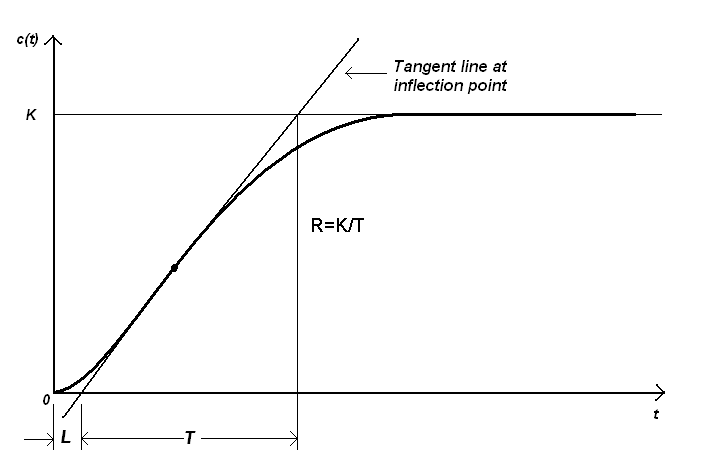
\includegraphics[width=\linewidth]{pid_manual/ReacCurve}
\caption{Reaction Curve\cite{kmmdc09}}
\label{RC}
\end{figure}
Ziegler-Nichols give rule for determining the values of gain $K$, integral time $\tau_i$ and derivative time $\tau_d$ based on the step response characteristics of a given plant.In this method one can experimentally obtain the response of a plant to a step input, as shown in figure \ref{RC}. This method is applicable only when the response to the step input exhibits S-shaped curve.\cite{ogt05}\\
As shown in figure \ref{RC}, by drawing the tangent line at the inflection point and determining the intersection of the tangent line with the time axis and the line $c(t)= K$ ,we get two constants, namely, delay time $L$ and time constant $T$.

Ziegler and Nichols suggested to set the values of $K, \tau_i , \tau_d$  according the formula shown in table \ref{table}.
\begin{table}
\begin{center}
\renewcommand{\arraystretch}{1.5}
\begin{tabular}{|c|r|r|r|}\hline
Type of
controller & $K$ & $\tau_i$ & $\tau_d$ \\ \hline
$P$ & $\frac{1}{RL}$ & $\infty$ & 0 \\ \hline
$PI$ & $\frac{0.9}{RL}$ & $3L$ & 0 \\\hline
$PID$ & $\frac{1.2}{RL}$ & $2L$ & $0.5L$ \\ \hline
\end{tabular}
\caption{Ziegler-Nichols tuning rule based on step response of plant}
\label{table}
\end{center}
\end{table}
Notice that the PID controller tuned by the Ziegler-Nichols rule gives,
\begin{align}
G_c(s)&=K_p\left(1+\frac 1{T_is}+T_ds\right)\\
&=1.2\frac {T}{L}\left( 1+\frac 1{2Ls}+0.5Ls\right)\\
&=0.6T\frac{\left(s+\frac 1{L}\right)^2}{s}
\end{align}
Thus the PID controller has a pole at the origin and double zeros at $s= -1/L$.

\subsection{Second Method}
\begin{figure}
\centering
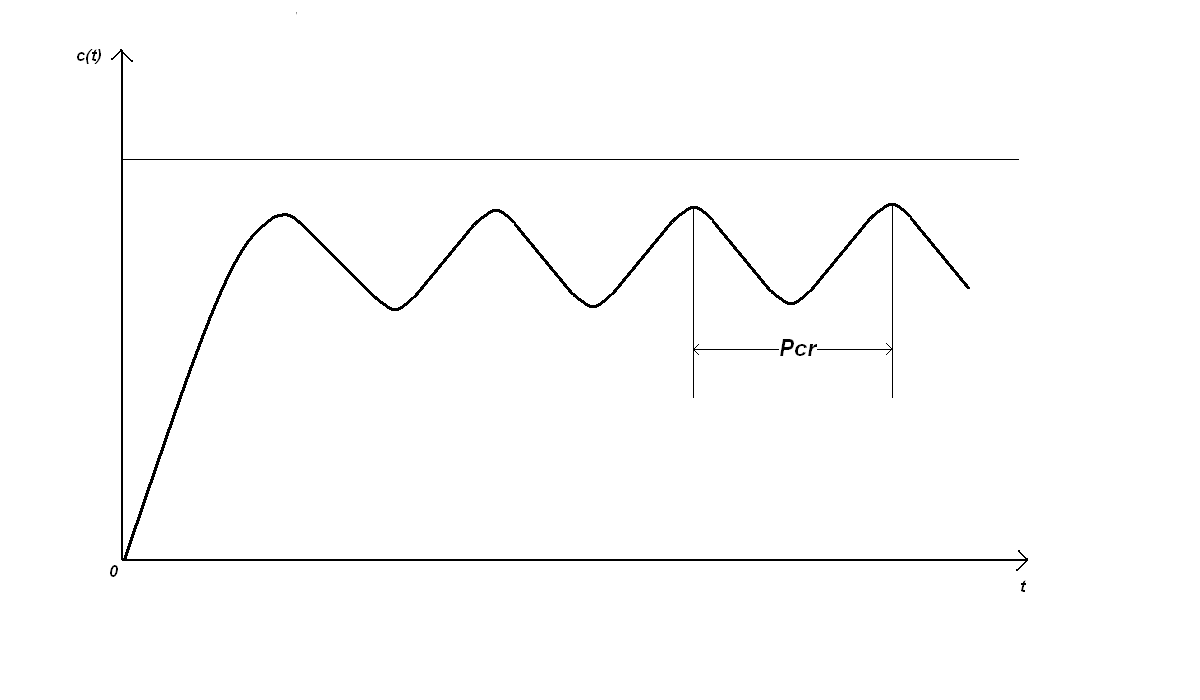
\includegraphics[width=\linewidth]{pid_manual/PIDUGtune}
\caption{Ziegler-Nichols instability tuning method}
\label{instability}
\end{figure}
The second method is also known as \textquoteleft instability method\textquoteright \cite{kmmdc09}. This is a closed loop method in which the Integral and Derivative gains of the PID controller are made zero with a unity value for proportional gain. A setpoint change is made and the temperature profile is observed for some time. The temperature would most likely maintain a steady-state with some offset. The gain is increased to a next distinct value (say 2) with a change in the setpoint. The procedure is repeated until the temperature first varies with sustained oscillations. It is necessary that the output (temperature) should have neither under damped nor over damped oscillations. At this particular frequency of sustained oscillations, the corresponding value of $K_p$ is noted and is called as the critical gain $K_{cr}$. The corresponding period of oscillation is known as  $P_{cr}$. Refer Fig. \ref{instability}.

The various P, PI and PID parameters are then calculated with the help of table \ref{2ndmtd}.
\begin{table}
\begin{center}
\renewcommand{\arraystretch}{1.5}
\begin{tabular}{|c|r|r|r|}\hline
Type of
controller & $K$ & $\tau_i$ & $\tau_d$ \\ \hline
$P$ & $0.5K_{u}$ & $\infty$ & 0 \\ \hline
$PI$ & $0.45K_{u}$ & $\frac{1}{0.2}P_{u}$ & 0 \\\hline
$PID$ & $0.6K_{u}$ & $0.5P_{u}$ & $0.125P_{u}$ \\ \hline
\end{tabular}
\caption{Ziegler-Nichols tuning rule for instability tuning method}
\label{2ndmtd}
\end{center}
\end{table}
\\
\\
\\
\\
Using the Ziegler-Nichols first method explained earlier, the following values were obtained. Refer figure \ref{steptest}.

\begin{figure}
\centering
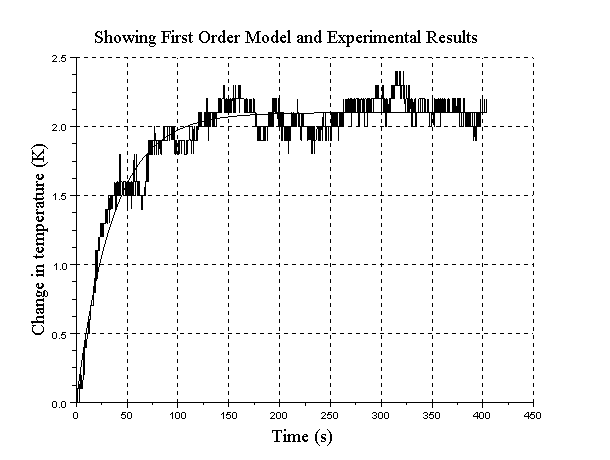
\includegraphics[width=0.7\linewidth]{pid_manual/forder_fit}
\caption{Refer \textquoteleft Step Test\textquoteright experiment\cite{kmm09}}
\label{steptest}
\end{figure}
\begin{align*}
L&=6\hspace{0.2cm}s\\
T&=193\hspace{0.2cm}s
\intertext{For PI}
K&=6.031\\
\tau _i&= 18\hspace{0.25cm}
\intertext{For PID}
K&=8\\
\tau _i&= 12\hspace{0.25cm}\\
\tau _d&= 3\hspace{0.25cm}
\end{align*}
While performing the experiment fine tunning of $K,\tau_i,\tau_d$ may be required.
\\

\section{Implementing PI controller using Trapezoidal Approximation}
Fig.\ref{pi_cos} shows Xcos for implementing PI controller.
\begin{figure}
\centering
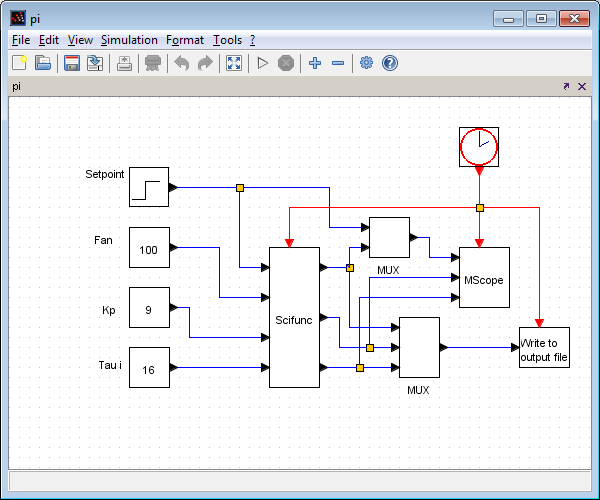
\includegraphics[width=0.7\linewidth]{pid_manual/pi_xcos.png}
\caption{Xcos for PI controller available as {\tt pi.xcos}}
\label{pi_cos}
\end{figure}
The PI controller in continuous time is given by 
\begin{align}
u(t)&=K \left\{e(t)+\frac{1}{\tau_i}\int_0^t e(t)dt\right\}
\intertext {On taking the Laplace transforms,we obtain}
u(t)&=K\left\{1+\frac 1{\tau_i s}\right\}e(t) \label{lt1}
\intertext{By mapping controller given in Eq.\ref{lt1} to the discrete time domain using  trapezoidal approximation}
u(n)&=K\left\{1+\frac{T_s}{2\tau_i}\frac{z+1}{z-1}\right\}e(n)
\intertext{On cross multiplying,we obtain}
(z-1)u(n)&=K\left\{(z-1)+\frac{T_s}{2\tau_i}(z+1)\right\}e(n)
\intertext{We divide by $z$ and then by using shifting theorem we obtain}
u(n)-u(n-1)&=K\left\{e(n)-e(n-1)+\frac{T_s}{2\tau_i}e(n)+\frac{T_s}{2\tau_i}e(n-1)\right\}
\intertext{The PI controller is usually written as}
u(n)&=u(n-1)+s_0 e(n)+s_1e(n-1)
\intertext{Where}
s_0&=K\left(1+\frac{T_s}{2\tau_i}\right) \\
s_1&=K\left(-1+\frac{T_s}{2\tau_i}\right)
\end{align}
For implementing above PI controller, scilab code is given in {\tt pi\_ta.sci} file, listed at the end of this document. Change the current working directory to the folder {\tt pid\_controller}. Execute the file {\tt ser\_init.sce} with the appropriate com port number and then execute the file {\tt pi\_ta.sci} for loading the function. Run the xcos file {\tt pi\_ta.xcos}. Output of Xcos is shown in below fig.\ref{pi_ta}. Figure shows three plots. First subplot shows Setpoint and output temperature profile. Second sub plot shows control effort and third subplot shows error between setpoint and plant output.

\subsection{Implementing PI controller using Trapezoidal Approximation on SBHS, virtually}
The step by step procedure for conducting an experiment virtually is explained in section \ref{vlabsexpt}. The required .sce file is {\tt pi\_ta\_virtual.sce}.  You will find this file in the {\tt pid\_controller} directory under {\tt virtual} folder.  The necessary codes are listed in the section \ref{pidcodes}

\begin{figure}
\centering
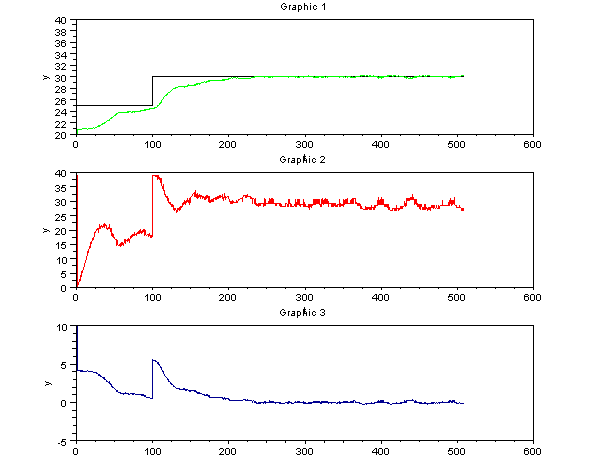
\includegraphics[width=0.6\linewidth]{pid_manual/pi_ta}
\caption{PI controller (Trapezoidal Approximation) output}
\label{pi_ta}
\end{figure}
 
\section{Implementing PI controller using Backward Difference Approximation}
The PI controller in continuous time is given by 
\begin{align}
u(t)&=K \left\{e(t)+\frac{1}{\tau_i}\int_0^t e(t)dt\right\}
\intertext {On taking the Laplace transform,we obtain}
u(t)&=K\left\{1+\frac 1{\tau_i s}\right\}e(t) \label{lt2}
\intertext{By mapping controller given in Eq.\ref{lt2} to the discrete time domain using  Backward difference approximation :}
u(n)&=K\left\{1+\frac{T_s}{\tau_i}\frac{z}{z-1}\right\}e(n)
\intertext{On cross multiplying,we obtain}
(z-1)u(n)&=K\left\{(z-1)+\frac{T_s}{\tau_i}(z)\right\}e(n)
\intertext{We divide by $z$ and then by using shifting theorem we obtain}
u(n)-u(n-1)&=K\left\{e(n)-e(n-1)+\frac{T_s}{\tau_i}e(n)\right\}
\intertext{The PI controller is usually written as}
u(n)&=u(n-1)+s_0 e(n)+s_1e(n-1)
\intertext{Where}
s_0&=K\left(1+\frac{T_s}{\tau_i}\right) \\
s_1&=-K
\end{align}
For implementing above PI controller scilab code is given in {\ttfamily pi\_bda.sci} file, listed at the end of this document. Change the current working directory to the folder {\tt pid\_controller}. Execute the file {\tt ser\_init.sce} with the appropriate com port number and then execute the file {\tt pi\_bda.sci} for loading the function. Run the xcos file {\tt pi\_bda.xcos}.Output of Xcos is shown in below fig.\ref{pi_bda}
\begin{figure}
\centering
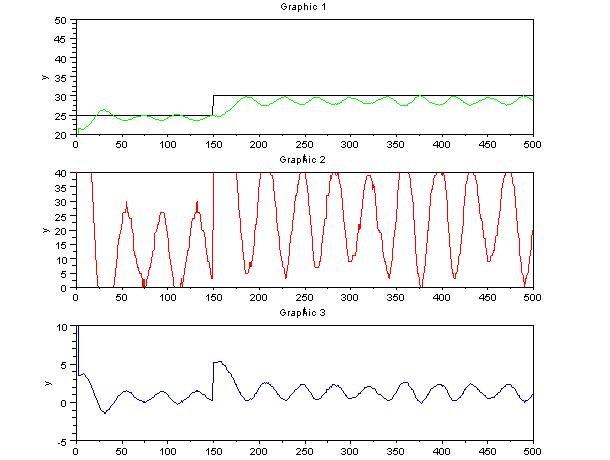
\includegraphics[width=0.6\linewidth]{pid_manual/pi_bda.jpg}
\caption{PI controller (Backward Difference Approximation) output}
\label{pi_bda}
\end{figure}
Figure shows three plots. First subplot shows Setpoint and output temperature profile. Second sub plot shows control effort and third subplot shows error between setpoint and plant output.

\subsection{Implementing PI controller using Backward Difference Approximation on SBHS, virtually}
The step by step procedure for conducting an experiment virtually is explained in section \ref{vlabsexpt}. The required .sce file is {\tt pi\_bda\_virtual.sce}.  You will find this file in the {\tt pid\_controller} directory under {\tt virtual} folder.  The necessary codes are listed in the section \ref{pidcodes}

\section{Implementing PI controller using Forward Difference Approximation}
The PI controller in continuous time is given by 
\begin{align}
u(t)&=K \left\{e(t)+\frac{1}{\tau_i}\int_0^t e(t)dt\right\}
\intertext {On taking the Laplace transforms,we obtain}
u(t)&=K\left\{1+\frac 1{\tau_i s}\right\}e(t) \label{lt3}
\intertext{By mapping controller given in Eq.\ref{lt3} to the discrete time domain using forward difference formula :}
u(n)&=K\left\{1+\frac{T_s}{\tau_i}\frac{1}{z-1}\right\}e(n)
\intertext{On cross multiplying,we obtain}
(z-1)u(n)&=K\left\{(z-1)+\frac{T_s}{\tau_i}\right\}e(n)
\intertext{We divide by $z$ and then by using shifting theorem we obtain}
u(n)-u(n-1)&=K\left\{e(n)-e(n-1)+\frac{T_s}{\tau_i}e(n-1)\right\}
\intertext{The PI controller is usually written as}
u(n)&=u(n-1)+s_0 e(n)+s_1e(n-1)
\intertext{Where}
s_0&=K \\
s_1&=K\left(-1+\frac{T_s}{\tau_i}\right)
\end{align}
For implementing above PI controller scilab code is given in {\ttfamily pi\_fda.sci} file, listed at the end of this document. Change the current working directory to the folder {\tt pid\_controller}. Execute the file {\tt ser\_init.sce} with the appropriate com port number and then execute the file {\tt pi\_fda.sci} for loading the function. Run the xcos file {\tt pi\_fda.xcos}.Output of Xcos is shown in below fig.\ref{pi_fda}
\begin{figure}
\centering
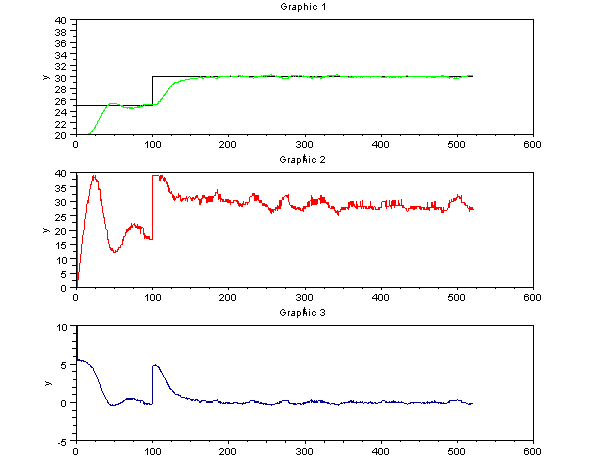
\includegraphics[width=0.6\linewidth]{pid_manual/pi_fda}
\caption{PI controller implementation (forward difference approximation)}
\label{pi_fda}
\end{figure}
 Figure shows three plots. First subplot shows Setpoint and output temperature profile. Second sub plot shows control effort and third subplot shows error between setpoint and plant output.


\subsection{Implementing PI controller using forward Difference Approximation on SBHS, virtually}
The step by step procedure for conducting an experiment virtually is explained in section \ref{vlabsexpt}. The required .sce file is {\tt pi\_fda\_virtual.sce}.  You will find this file in the {\tt pid\_controller} directory under {\tt virtual} folder.  The necessary codes are listed in the section \ref{pidcodes}

\section{Implementing PID controller  using Backward difference approximation}
Fig.\ref{pid_cos} shows Xcos for implementing PID controller .
\begin{figure}
\begin{center}
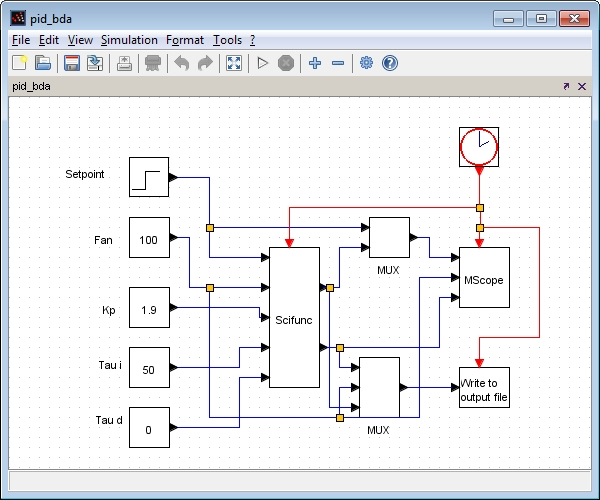
\includegraphics[width=0.6\linewidth]{pid_manual/pid_bda_xcos.jpg}
\caption{Xcos for PID controller available as {\tt pid\_bda.xcos}}
\label{pid_cos}
\end{center}
\end{figure}
The PID controller in continuous time is given by 
\begin{align}
u(t)&=K \left\{e(t)+\frac{1}{\tau_i}\int_0^t e(t)dt+\tau_d\frac{de(t)}{dt}\right\}
\intertext {On taking the Laplace transforms,we obtain}
u(t)&=K\left\{1+\frac 1{\tau_i s}+\tau_d s\right\}e(t) \label{lt4}
\intertext{By mapping controller given in Eq.\ref{lt4} to the discrete time domain using backward difference formula :}
u(n)&=K\left\{1+\frac{T_s}{\tau_i}\frac{z}{z-1}+\frac{\tau_d}{T_s}\frac{z-1}{z}\right\}e(n)
\intertext{On cross multiplying,we obtain}
(z^2-z)u(n)&=K\left\{(z^2-z)+\frac{T_s}{\tau_i}z^2+\frac{\tau_d}{T_s}(z-1)^2\right\}e(n)
\intertext{We divide by $z^2$ and by using shifting theorem we obtain}
u(n)-u(n-1)&=K\left\{e(n)-e(n-1)+\frac{T_s}{\tau_i}e(n)\right.\nonumber \\
\hspace{1cm}&+ \left. \frac{\tau_d}{T_s}[e(n)-2e(n-1)+e(n-2)]\right\}
\intertext{The PID controller is usually written as}
u(n)&=u(n-1)+s_0 e(n)+s_1e(n-1)+s_2e(n-2)
\intertext{Where}
s_0&=K\left[1+\frac{T_s}{\tau_i}+\frac{\tau_d}{T_s}\right] \\
s_1&=K\left[-1-2\frac{\tau_d}{T_s}\right]\\
s_2&=K\left[\frac{\tau_d}{T_s}\right]
\end{align}
For implementing above PID controller scilab code is given in {\tt pid\_bda.sci} file,listed at the end of this document. Change the current working directory to the folder {\tt pid\_controller}. Execute the file {\tt ser\_init.sce} with the appropriate com port number and then execute the file {\tt pid\_bda.sci} for loading the function. Run the xcos file {\tt pid\_dda.xcos}. Output of Xcos is shown in below fig.\ref{pid_bda}
\begin{figure}
\centering
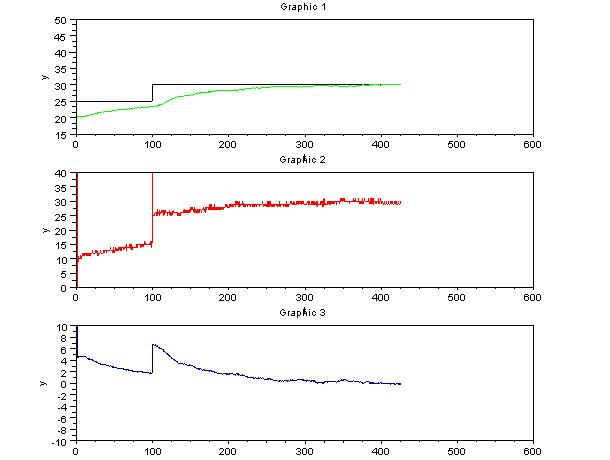
\includegraphics[width=0.7\linewidth]{pid_manual/pid_bda_graph}
\caption{PID controller (Backward Difference Approximation) Output}
\label{pid_bda}
\end{figure}
 Figure shows three plots. First subplot shows Setpoint and output temperature profile. Second sub plot shows control effort and third subplot shows error between setpoint and plant output.

\subsection{Implementing PID controller using backward Difference Approximation on SBHS, virtually}
The step by step procedure for conducting an experiment virtually is explained in section \ref{vlabsexpt}. The required .sce file is {\tt pid\_bda\_virtual.sce}.  You will find this file in the {\tt pid\_controller} directory under {\tt virtual} folder.  The necessary codes are listed in the section \ref{pidcodes}

\section{Implementing PID controller using trapezoidal approximation for integral mode and Backward difference approximation for the derivative mode}
The PID controller in continuous time is given by 
\begin{align}
u(t)&=K \left\{e(t)+\frac{1}{\tau_i}\int_0^t e(t)dt+\tau_d\frac{de(t)}{dt}\right\}
\intertext {On taking the Laplace transforms,we obtain}
u(t)&=K\left\{1+\frac 1{\tau_i s}+\tau_d s\right\}e(t) \label{lt5}
\intertext{By mapping controller given in Eq.\ref{lt5} to the discrete time domain using trapezoidal approximation for integral mode and Backward difference approximation for the derivative mode}
u(n)&=K\left\{1+\frac{T_s}{2\tau_i}\frac{z+1}{z-1}+\frac{\tau_d}{T_s}\frac{z-1}{z}\right\}e(n)
\intertext{On cross multiplying,we obtain}
(z^2-z)u(n)&=K\left\{(z^2-z)+\frac{T_s}{2\tau_i}(z^2+z)\frac{\tau_d}{T_s}(z-1)^2\right\}e(n)
\intertext{We divide by $z^2$ and then by using shifting theorem we obtain}
u(n)-u(n-1)&=K\left\{e(n)-e(n-1)+\frac{T_s}{2\tau_i}{e(n)+e(n-1)}\right.\nonumber \\
\hspace{1cm}&+ \left. \frac{\tau_d}{T_s}[e(n)-2e(n-1)+e(n-2)]\right\}
\intertext{The PID controller is usually written as}
u(n)&=u(n-1)=s_0 e(n)+s_1e(n-1)+s_2e(n-2)
\intertext{Where}
s_0&=K\left[1+\frac{T_s}{2\tau_i}+\frac{\tau_d}{T_s}\right] \\
s_1&=K\left[-1+\frac{T_s}{2\tau_i}-2\frac{\tau_d}{T_s}\right]\\
s_2&=K\frac{\tau_d}{T_s}
\end{align}
For implementing above PID controller scilab code is given in {\tt pid\_ta\_bda.sci} file,listed at the end of this document. Change the current working directory to the folder {\tt pid\_controller}. Execute the file {\tt ser\_init.sce} with the appropriate com port number and then execute the file {\tt pid\_ta\_bda.sci} for loading the function. Run the xcos file {\tt pid\_ta\_bda.xcos}.
Output of Xcos is shown in below fig.\ref{pid_ta_bda}
\begin{figure}
\centering
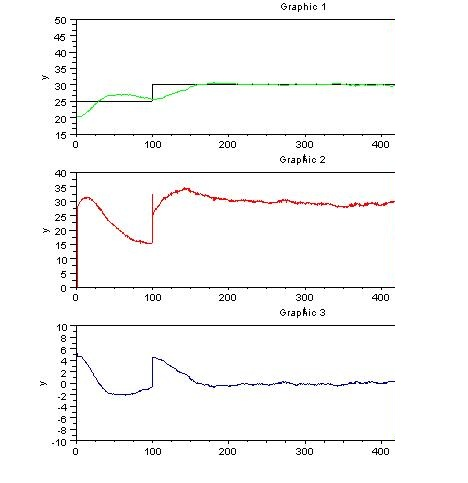
\includegraphics[width=0.6\linewidth]{pid_manual/pid_ta_bda_graph.jpg}
\caption{PID controller (TA - BDA) implementation}
\label{pid_ta_bda}
\end{figure}
 Figure shows three plots. First subplot shows Setpoint and output temperature profile. Second sub plot shows control effort and third subplot shows error between setpoint plant output i.e. temperature.

\subsection{Implementing PID controller using trapezoidal approximation for integral mode and Backward difference approximation for the derivative mode on SBHS, virtually}
The step by step procedure for conducting an experiment virtually is explained in section \ref{vlabsexpt}. The required .sce file is {\tt pid\_ta\_bda\_virtual.sce}.  You will find this file in the {\tt pid\_controller} directory under {\tt virtual} folder.  The necessary codes are listed in the section \ref{pidcodes}

Due to the introduction of derivative action control effort shows lots of fluctuations. By using filtered form of PID we can make derivative mode implementable.


\section{Implementing PID controller with filtering using Backward difference approximation}
Fig.\ref{pid_filter_xcos} shows Xcos for implementing PID controller with filtering
\begin{figure}
\begin{center}
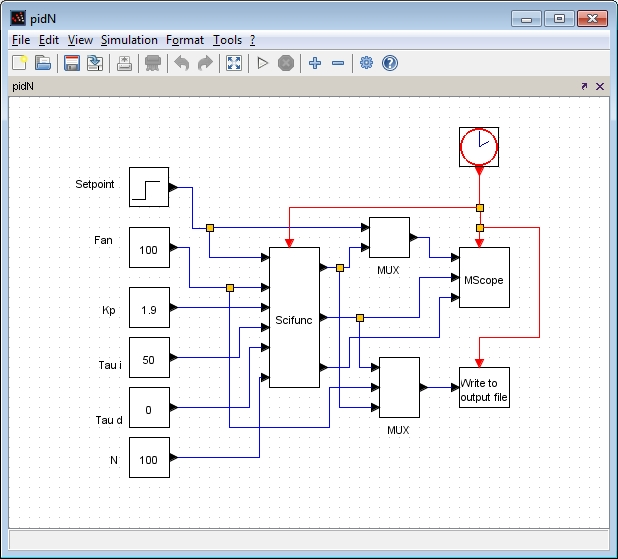
\includegraphics[width=0.6\linewidth]{pid_manual/pidN}
\caption{Xcos for PID controller with filtering available as {\tt pidN.xcos}}
\label{pid_filter_xcos}
\end{center}
\end{figure}
\begin{align}
\intertext{PID filtered form is given by}
u(t)&=K\left\{1+\frac 1{\tau_i s}+\frac{\tau_d s}{1+\frac{\tau_d s}{N}}\right\}e(t) \label{lt6}
\intertext{Where N is large number,of the order of 100. By maping controller given in Eq.\ref{lt6} to the discrete 
time domain using backward difference formula :}
u(n)&=K\left(1+\frac{T_s}{\tau_i}\frac{1}{1-z^{-1}}+\frac{\tau_d (1-z^{-1})}{1+\frac{\tau_d(1-z^{-1})}{N}}\right)e(n)\\
u(n)&=K\left(1+\frac{T_s}{\tau_i}\frac{1}{1-z^{-1}}+\frac{Nr_1(1-z^{-1})}{1+r_1z^{-1}}\right)e(n)
\intertext{Where}
r_1&=-\frac{\frac{\tau_d}{N}}{\frac{\tau_d}{N}+T_s}
\intertext{On cross multiplying,we obtain}
(1-z^{-1})(1+r_1 z^{-1})u(n)&=K[(1-z^{-1})(1+r_1 z^{-1})\nonumber\\
&+\frac{T_s}{\tau_i}(1+r_1z^{-1})+\frac{\tau_d}{T_s}(1-z^{-1})^2]e(n)
\intertext{Simplifying and then by using shifting theorem we obtain}
u(n)+(r_1-1)u(n&-1)\nonumber\\
-r_1u(n&-2)=K\left[1+\frac{T_s}{\tau_i}-Nr_1\right]e(n)\nonumber\\
&+K\left[r_1(1+\frac{T_s}{\tau_i}+2N)-1\right]e(n-1)\nonumber\\
&-K\left[r_1(1+N)\right]e(n-2)\\
\intertext{hence}
u(n)&=r_1u(n-2)-(r_1-1)u(n-1)\nonumber\\
&+s_0 e(n)+s_1e(n-1)+s_2e(n-2)
\intertext{Where}
s_0&=K\left[1+\frac{T_s}{\tau_i}-Nr_1\right] \\
s_1&=K\left[r_1(1+\frac{T_s}{\tau_i}+2N)-1\right]\\
s_2&=-K\left[r_1(1+N)\right]
\end{align}
For implementing above PID controller scilab code is given in {\tt pid\_filter.sci} file,listed at the end of this document. Change the current working directory to the folder {\tt pid\_controller}. Execute the file {\tt ser\_init.sce} with the appropriate com port number and then execute the file {\tt pid\_filter.sci} for loading the function. Run the xcos file {\tt pidN.xcos}. Output of Xcos is shown in below fig.\ref{pid_filter}
\begin{figure}
\centering
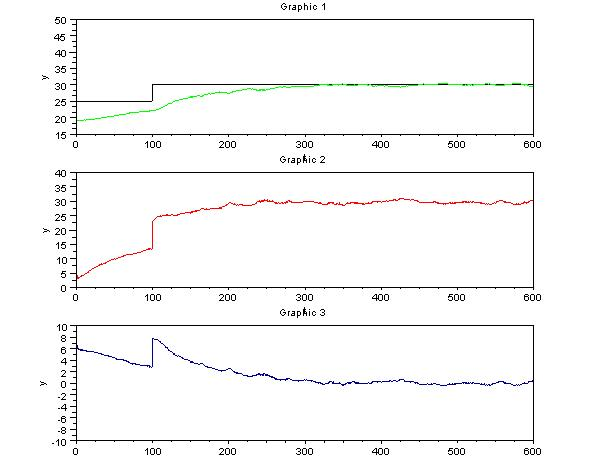
\includegraphics[width=0.7\linewidth]{pid_manual/pid_filter.jpg}
\caption{PID controller (with filtering) implementation}
\label{pid_filter}
\end{figure}
 Figure shows three plots. First subplot shows Setpoint and output temperature profile. Second sub plot shows control effort and third subplot shows error between setpoint and plant output.
By comparing fig.\ref{pid_bda} and fig.\ref{pid_filter} it is clear that introduction of filtered form of PID reduces fluctuations in control effort.

\subsection{Implementing PID controller with filtering using Backward difference approximation on SBHS, virtually}
The step by step procedure for conducting an experiment virtually is explained in section \ref{vlabsexpt}. The required .sce file is {\tt pid\_filter\_virtual.sce}.  You will find this file in the {\tt pid\_controller} directory under {\tt virtual} folder. The necessary codes are listed in the section \ref{pidcodes}


\section{Scilab Code}\label{pidcodes}
\subsection{Scilab code for serial communication}
%\addtocontents{cod}{\protect\addvspace{\codclr}}
\begin{code}
\ccaption{ser\_init.sci}{ser\_init.sci used for serial communication}
\lstinputlisting{Scilab/local/pid_controller/ser_init.sce}
\end{code}
\subsection{Scilab code for PI controller}
\begin{code}
\ccaption{pi\_ta.sci}{pi\_ta.sci}
\lstinputlisting{Scilab/local/pid_controller/pi_ta.sci}
\end{code}
\begin{code}
\ccaption{pi\_bda.sci}{ pi\_bda.sci}
\lstinputlisting{Scilab/local/pid_controller/pi_bda.sci}
\end{code}
\begin{code}
\ccaption{pi\_fda.sci}{ pi\_fda.sci}
\lstinputlisting{Scilab/local/pid_controller/pi_fda.sci}
\end{code}
\subsection {Scilab code for PID controller}
\begin{code}
\ccaption{pid\_bda.sci}{ pid\_bda.sci}
\lstinputlisting{Scilab/local/pid_controller/pid_bda.sci}
\end{code}
\begin{code}
\ccaption{pid\_ta\_bda.sci}{ pid\_ta\_bda.sci}
\lstinputlisting{Scilab/local/pid_controller/pid_ta_bda.sci}
\end{code}
\begin{code}
\ccaption{pid\_filter.sci}{ pid\_filter.sci}
\lstinputlisting{Scilab/local/pid_controller/pid_filter.sci}
\end{code}

\begin{code}
\ccaption{pid\_bda\_virtual.sce}{pid\_bda\_virtual.sce}
\lstinputlisting{Scilab/virtual/pid_controller/pid_bda_virtual.sce}
\end{code}

\begin{code}
\ccaption{pid\_bda\_virtual.sci}{pid\_bda\_virtual.sci}
\lstinputlisting{Scilab/virtual/pid_controller/pid_bda_virtual.sci}
\end{code}

%\bibliography{pid}
